% ORSSEY
\section{Wielomiany Alexandera}

Wiele wskazuje na to, że niebawem teoria węzłów będzie przeżywać drugą młodość. Na początku chciano ją wykorzystać do opisywania mikroświata. Jak się okazało, nie odpowiadała ona
fizycznym własnościom rzeczywistości, jednak został rozwinięty aparat matematyczny. Jak wiadomo DNA wszystkich żywych organizmów jest poskręcane, a dodatkowo DNA bakterii ma strukturę splotu węzłów.
Całkiem niedawno odkryto, że w momencie kiedy bakteria chce się podzielić musi przeciąć
nic DNA wzdłuż (taka nic nie ma wolnych końców) i wtedy mogą powstawać supły. Dzięki takim supłom replikacja bakterii byłaby niemożliwa, ale pod wpływem enzymu zwanego topoizomerazą bakteria jest w stanie
rozsupłać węzły. Biolodzy wspólnie z matematykami badają topologiczne własności takich struktur i mechanizmy, które za tym stoją, aby je zakłócić i tym samym uniemożliwić rozmnażanie się bakteriom.


%--------------------------------------
 

\subsection{Wielomian Laurenta}

Formalne wprowadzenie wielomianów Alexandera można zrealizować na kilka sposobów. Jednym z nich jest wykorzystanie do tego pojęcia wielomianów HOMFLY - uogólnionych wielomianów Jonesa.
Innym sposobem jest
użycie formalizmów topologii algebraicznej. Wtedy pewne cięcia i sklejania powierzchni Seiferta determinują wielomian Alexandera. To właśnie ta metodologia
pozwoliła po raz pierwszy udowodnić prawdziwość twierdzeń Alexandera. 

Poniżej wprowadzimy pojęcie wielomianów Alexandera elementarnie, skupiając się
na procedurze ich wyznaczania i pokażemy niezależność od ruchów Reidemeistera. Dodatkowo zdefiniuemy je jako pewną funkcję węzła.
Jednak żeby zachować formalizm wpierw zdefiniujemy pojęcie wielomianów Laurenta.

\begin{definicja}
   Wielomian Laurenta zmiennej X jest symbolem postaci:

   $$
   f = a_rX^r + a_{r+1}X^{r+1} + \dots + a_sX^s
   $$

   gdzie $r \leqslant s$ ($r, s \in \mathbb{Z}$, dopuszczalne są wartość ujemne) oraz $a_r \dots a_s \in \mathbb{Z}$.
   Jeżeli wartość $a_r = 0$ to jako $f$ przyjmujemy $a_{r+1}X^{r+1} + \dots + a_sX^s$.
   Podobnie gdy $a_s = 0$.
   Wielomian ten podlega zwykłym działaniom dodawania i mnożenia wielomianów.
   Zbiór wszystkich wielomianów Laurenta zmiennej $X$ oznaczany jest jako $\mathbb{Z}[X, X^{-1}]$.
   Aby podkreślić od jakiej zmiennej zależy wielomian $f$ czasami będziemy pisać $f(X)$.
\end{definicja}

Wielomian Alxandera, który zdefiniujemy poniżej będzie wielomianem Laurenta zmiennej $t$, tzn
będzie elementem zbioru $\mathbb{Z}[t , t^{-1}]$. Piszemy $f(t) \stackrel{\bullet}{=} g(t)$ jeżeli $f(t) = \pm t^mg(t)$
dla pewnego $m \in \mathbb{Z}$.


%--------------------------------------


\subsection{Macierz skrzyżowań}

Aby obliczyć wielomian Alexandera $\Delta_L(t)$ węzła $L$ (czasem będziemy pisali $\Delta(L)$), wpierw ustalamy dla niego zorientowany diagram $D$ bez krzywych zamkniętych.
Następnie etykietujemy $D$, tzn przypisujemy pewne unikalne wartości (np.: liczby lub litery)
dla łuków i skrzyżowań. W węźle występują dwa rodzaje skrzyżowań: prawozorientowane i lewozorientowane. 

\begin{center}
   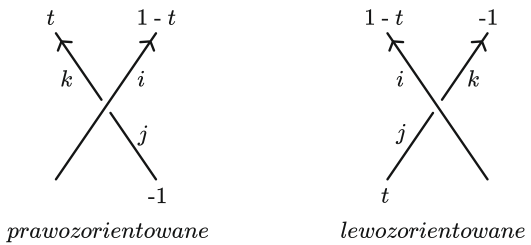
\includegraphics[scale=0.5]{3/images/1}
\end{center}

Orientację skrzyżowania wyznacza kierunek nadrzędnego łuku. Dla pierwszego skrzyżowania z Rysunku 1. łuk przechodzący nad przechodzi ze strony lewej do prawej, czyli jest prawozorientowany, 
analogicznie dla skrzyżowania lewozorientowanego.

\begin{definicja}
   Zdefinujemy macierz $A_+$ wymiaru $n \times n$, gdzie $n$ jest liczbą skrzyżowań (i łuków - zobacz dowód Lematu 3.13) według poniższej procedury. Powtórzymy
   ją dla każdego skrzyżowania $l$ w węźle:

   \begin{enumerate}
   \item Jeśli skrzyżowanie $l$ jest prawozorientowane i łuk $i$ przechodzi nad łukami $j$, $k$ (Rysunek 1.), to w wierszu $l$ wpisujemy $1 - t$ w kolumnie $i$, $-1$ w kolumnie $j$ oraz $t$ w kolumnie $k$
   \item Jeśli skrzyżowanie $l$ jest lewozorientowane i łuk $i$ przechodzi nad łukami $j$, $k$ (Rysunek 1.), to w wierszu $l$ wpisujemy $1-t$ w kolumnie $i$, $t$ w kolumnie $j$ oraz $-1$ w kolumnie $k$
   \end{enumerate}

   Wszystkie pozostałe wyrazy w wierszu $l$ są równe 0. Może się zdarzyć przypadek, kiedy jakieś $i, j, k$ są tym samym łukiem. Wtedy we właściwej kolumnie wpisujemy sumę wyrazów opisanych powyżej.
   Dla przykładu (Rysunek 2.), jeżeli $j=k$ dla jakiegoś lewozorientowanego skrzyżowania, to wpisujemy $-1+t$ w kolumnie $j$ ($=k$).

   \begin{center}
      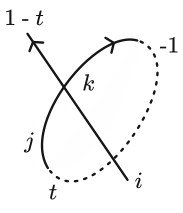
\includegraphics[scale=0.5]{3/images/2}
   \end{center}
\end{definicja}

\begin{wniosek}
   Jeżeli przyjmiemy $t = -1$ to dostaniemy macierz standardowych równanań kolorujących.
\end{wniosek}

\begin{proof}
   Dowód polega na porównaniu definicji $\Delta_L$ i $\det(L)$.
\end{proof}

\begin{przyklad}
   Pokażemy bardzo elementarnie na przykładzie trójliścia jak wyznaczyć macierz.
   Nadajemy etykiety dla skrzyżowań i łuków. Następnie rozpoznajemy orientację skrzyżowań. Narysujemy zatem rozpatrywany węzeł w taki sposób,
   by każde skrzyżowanie odpowiadało jednemu z Rysunku 1.

   \begin{center}
      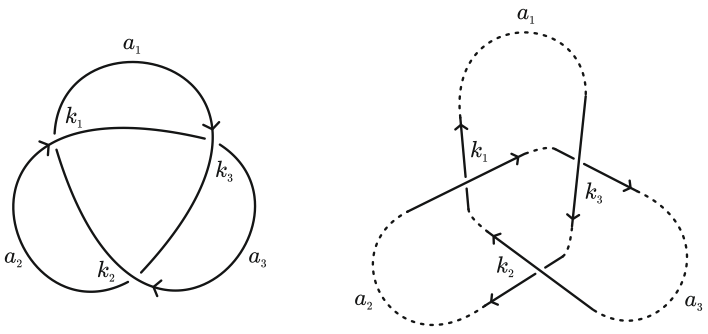
\includegraphics[scale=0.5]{3/images/3}
   \end{center}

   Przyjrzymy się teraz samym skrzyżowaniom. Wielomiany przyporządkujemy zgodnie z podaną procedurą.
   
   \begin{center}
      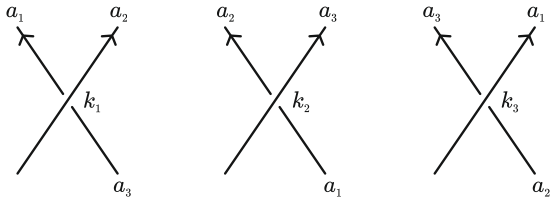
\includegraphics[scale=0.5]{3/images/4}
   \end{center}

   Wtedy odpowiadająca jemu macierz wygląda następująco:
   
   $$
   A_+ = 
   \left( \begin{array}{ccc}
   t & 1-t & -1 \\
   -1 & t & 1-t \\
   1-t & -1 & t
   \end{array} \right)
   $$ 
\end{przyklad}


%--------------------------------------


\subsection{Macierz  i wielomian Alexandera}

\begin{definicja}
   Macierz $A$ wymiaru $(n-1) \times (n-1)$ powstała poprzez usunięcie dowolnego wiersza i dowolnej kolumny z macierzy $A_+$
   nazywamy macierzą Alexandera węzła $L$. Wyznacznik macierzy Alexandera jest nazywany wielomianem Alexandera węzła $L$ i oznaczany przez $\Delta_L(t)$ ($\Delta(L)$).
   Wyznacznik macierzy $0 \times 0$ definiujemy jako $1$.
   
   $\newline$
   
   Jeżeli nie zostanie powiedziane inaczej macierz Aleksandera $A$ będzie minorem $A_+^{(1,1)}$.
\end{definicja}

\begin{przyklad}
   Wielomian Alexandera dla przykładu - trójliścia wynosi $\Delta_3(t) = t^2 - t + 1$. Aby się przekonać obliczymy wyznacznik macierzy $A_+^{(3,1)}$:

   $$
   \Delta_3(t) = \det \left( \begin{array}{ccc}
   1-t & -1 \\
   t & 1-t
   \end{array} \right) = (1-t)^2 - (-t) = 1 + t^2 -2t + t = t^2 - t + 1  
   $$ 
\end{przyklad}

\begin{wniosek}
   Wielomian Alexandera nie zależy od tego, który wiersz i którą kolumnę usuniemy.
\end{wniosek}  

\begin{proof}
   Pokażemy, że wyznacznik macierzy powstałej przez usunięcie $j$-kolumny oraz $i$-wiersza trzyma w relacji $\stackrel{\bullet}{=}$ wyznacznik minora $(1,1)$.
   
   $$
   \det A^{(1,1)} = \det( A_2^{(1)}, A_3^{(1)}, \cdots , A_n^{(1)} )
   $$

   Rozważmy wyznacznik macierzy $\det A^{(1, j)} = \det (A_1^{(1)}, A_2^{(1)}, \cdots, A_{j-1}^{(1)}, A_{j+1}^{(1)}, \cdots,  A_n^{(1)})$.
   Korzystajac z tego, że suma wierszy oraz kolumn wynosi $0$, możemy do $A_1^{(1)}$ dodać pozostałe kolumny otrzymując
   $\det A^{(1, j)} = \det (-A_j^{(1)}, A_2^{(1)}, \cdots, A_{j-1}^{(1)}, A_{j+1}^{(1)}, \cdots, A_n^{(1)})$. Odpowiednia liczba transpozycji kolumn i wyciągnięcie $-1$ z $A_j^{(1)}$ daje 
   $$
      \det A^{(1, j)} = (-1)^{j+1} \det A^{(1,1)}
   $$
   
   Podobnie postępujemy z wierszami i ostatecznie
   
   $$\det A^{(i, j)} = (-1)^{(i+1+j+1)} \det A^{(1,1)} =  (-1)^{(i+j)} \det A^{(1,1)} \stackrel{\bullet}{=} \det A^{(1,1)}$$
\end{proof}

\begin{przyklad}
   Obliczając wyznacznik macierzy $A_+^{(1,2)}$ dla trójliścia z przykładu powyżej dostaniemy $\Delta_3'(t) = -(t^2 - t + 1)$, czyli  $-\Delta_3(t)$.
\end{przyklad}

Podczas wyznaczania wielomianu Alexandera dokonaliśmy wyborów, które mają wpływ na postać wielomianu, tj:
wybór diagramu, etykietowanie łuków i skrzyżowań. Rożne wybory mogą prowadzić do różnych wielomianów Alexandera.

\begin{twierdzenie}
   Klasa równoważności relacji $\stackrel{\bullet}{=}$ wielomianów Alexandra $\Delta_L(t)$ jest dobrze zdefiniowanym
   niezmiennikiem zorientowanych węzłów, tzn relacja $\Delta_L^1(t) \stackrel{\bullet}{=} \Delta_L^2(t)$ jest zawsze utrzymana.
\end{twierdzenie}

\begin{proof}
   Twierdzenie to jest analogiczne do tego, że wyznacznik (zobacz <a href="">rodział kolorowań</a>) jest niezmiennikiem węzła.
   Ten fakt opiera się na zależności pomiędzy wyznacznikiem, a grupą kolorowań. 
   Moglibyśmy powyższe twierdzenie szybko udowodnić przytaczając zależność 
   pomiędzy wielomianem Alexandera, a obiektem zwanym modułem Alexandera, tzn modułem pierścienia $\mathbb{Z}[t, t^{-1}]$. 
   Nie chcemy się zagłębiać w teorię modułów, więc powyższe twierdzenie udowodnimy sprawdzając, że po wykonaniu ruchów Reidemeistera wielomian pozostaje w relacji $\stackrel{\bullet}{=}$.
   
   $\newline$
   
   Przy dowodzeniu za pomocą ruchów Reidemeistera patrzymy jak zmienia się wyznacznik po wykonaniu ruchu.
   
   \begin{enumerate}
      \item I ruch Reidemeistera
         
         $\newline$

         Można założyć bez straty ogólności, że ruch jest wykonywamy pomiędzy skrzyżowaniami $x$ i $y$ na $k$-łuku. Macierz $A_+$ jest wymiaru $n \times n$. Macierz $A$ uzyskamy
         usuwając pierwszy wiersz i pierwszą kolumnę.
         
         $$ 
          A_+ =  \begin{pmatrix}
         A_{1,1} & \cdots & A_{1,n-1} & k_1 \cr
         A_{2,1} & \cdots & A_{2,n-1} & k_2 \cr
          \vdots & \vdots & \cdots    & \vdots \cr
         A_{x,1} & \cdots & A_{x,n-1} & k_x \cr
         A_{y,1} & \cdots & A_{y,n-1} & k_y 
         \end{pmatrix}, \qquad A =          
         \begin{pmatrix}
         A_{2,2} & \cdots & A_{2,n-1} & k_2 \cr
          \vdots & \vdots & \cdots    & \vdots \cr
         A_{x,2} & \cdots & A_{x,n-1} & k_x \cr
         A_{y,2} & \cdots & A_{y,n-1} & k_y 
         \end{pmatrix}
         $$
         
         Wykonanie I ruchu Reidemeistera dodaje nowe skrzyżowanie (dodajemy jako ostatni wiersz), co wiąże się ze zmianą etykiet łuków.
         Pewna część kolumny $k$-łuku pozostanie bez zmian (oznaczymy ją przez $l$), pozostała część tej kolumny
         przejdzie na kolumnę łuku oznaczonego jako $m$. By nie ustalać kolejności etykietowania zauważamy zależność

         $$
         (*) \qquad \qquad \forall i \in I \quad k_i = l_i+ m_i,
         $$
         
         przy czym dokładnie jeden ze składników sumy jest równy $0$, a $I$ jest zbiorem etykiet skrzyżowań. Ruch ten powiększy wymiar macierzy do $n + 1$.
         
         $$
         A_+' =  \begin{pmatrix}
         A_{1,1} & \cdots & A_{1,n-1} & l_1 & m_1 \\
         A_{2,1} & \cdots & A_{2,n-1} & l_2 & m_2\\
         \vdots & \vdots & \cdots & \vdots \\
         A_{n-2,1} & \cdots & A_{n-2,n-1} & l_{n-2} & m_{n-2} \\
         A_{x,1} & \cdots & A_{x,n-1} & k_x & 0 \\
         A_{y,1} & \cdots & A_{y,n-1} & 0 & k_y \\
         0     & \cdots   &  0 & p(t) & -p(t)
         \end{pmatrix}
         $$
         
         gdzie $p(t), q(t) \in \{ -1,1,-t,t \}$ oraz $p(t)+q(t) = \pm (t-1)$. Następnie $m$-kolumnę dodajemy do $l$-kolumny.
         Zgodnie z $(*)$ dostajemy macierz, która po wykreśleniu pierwszej kolumny i pierwszego
         wiersza wygląda następująco:
         
         $$
         A' = \begin{pmatrix}
         A_{2,2} & \cdots & A_{2,n-1} & k_2 & m_2\\
         \vdots & \vdots & \cdots    & \vdots \\
         A_{n-2,2} & \cdots & A_{n-2,n-1} & k_{n-2} & m_{n-2} \\
         A_{x,2} & \cdots & A_{x,n-1} & k_x & 0 \\
         A_{y,2} & \cdots & A_{y,n-1} & k_y & k_y \\
         0     & \cdots   &    0      & 0 & -p(t)
         \end{pmatrix}
         $$
         
         Stosując rozwinięcie Laplace'a względem ostatniego wiersza otrzymujemy: 
         
         $$
         \det A = \Delta_L^1(t) \stackrel{\bullet}{=} \Delta_L^2(t) = \det A' = \pm p(t) \det A
         $$
   
   
      \item II ruch Reidemeistera
         
         $\newline$
         
         Ruch ten jest wykonywany na $l$-łuku, pomiędzy skrzyżowaniami $u$ i $v$ oraz $k$-łuku, pomiędzy skrzyżowaniami $x$ i $y$. Łukiem górnym jest $k$-łuk.
         Usuwamy pierwszy wiersz i pierwsza kolumnę otrzymując macierz $A$:
         
         $$
         A =  \begin{pmatrix}
         A_{2,2} & \cdots & A_{2,n-2} & k_2 & l_2 \\
         \vdots & \vdots & \cdots    & \vdots \\
         A_{n-4,2} & \cdots & A_{n-4,n-2} & k_{n-4} & l_{n-4} \\
         A_{x,2} & \cdots & A_{x,n-2} & k_x & 0 \\
         A_{y,2} & \cdots & A_{y,n-2} & k_y &0 \\
         A_{u,2} & \cdots & A_{u,n-2} & 0 & l_u \\
         A_{v,2} & \cdots & A_{v,n-2} & 0 & l_v
         \end{pmatrix}
         $$
         
         Po wykonaniu ruchu Reidemestera wymiar macierzy powiększy się o $2$. Zatem macierz Alexandera przyjmuje postać:
         
         $$
         A' = \begin{pmatrix}
         A_{2,2} & \cdots & A_{2,n-2} & k_2 & m_2 & o_2 & 0 \\
         \vdots & \vdots & \cdots    & \vdots & & & \vdots \\
         A_{n-4,2} & \cdots & A_{n-4,n-2} & k_{n-4} & m_{n-4} & o_{n-4} & 0  \\
         A_{x,2} & \cdots & A_{x,n-2} & k_x & 0 & 0 & 0 \\
         A_{y,2} & \cdots & A_{y,n-2} & k_y & 0 & 0 & 0 \\
         A_{u,2} & \cdots & A_{u,n-2} & 0 & l_u & 0 & 0 \\
         A_{v,2} & \cdots & A_{v,n-2} & 0 & 0 & l_v & 0 \\
         0 & \cdots & 0 & -p(t)-q(t) & p(t) & 0 & q(t) \\
         0 & \cdots & 0 & -p(t)-q(t) & 0 & p(t) & q(t) \\
         \end{pmatrix}
         $$
         
         
         gdzie dzięki $(*)$ zachodzi $l = m + o$. Wykonamy kolejno operacje macierzowe: od ostatniego wiersza odejmiemy wiersz przedostatni,
         do $m$-kolumny dodamy $o$-kolumnę, rozwiniemy względem ostatniego wiersza otrzymując:

         $$
         \det A' = 
         \pm p(t) \;  \det \begin{pmatrix}
         A_{2,2} & \cdots & A_{2,n-2} & k_2 & l_2 & 0 \\
          \vdots & \vdots & \cdots    & \vdots \\
         A_{n-4,2} & \cdots & A_{n-4,n-2} & k_{n-4} & l_{n-4} & 0  \\
         A_{x,2} & \cdots & A_{x,n-2} & k_x & 0 & 0 \\
         A_{y,2} & \cdots & A_{y,n-2} & k_y & 0 & 0 \\
         A_{u,2} & \cdots & A_{u,n-2} & 0 & l_u & 0 \\
         A_{v,2} & \cdots & A_{v,n-2} & 0 & l_v & 0 \\
         0 & \cdots & 0 & -p(t)-q(t) & p(t) & q(t)
         \end{pmatrix}
         $$
         
         Rozwijamy względem ostatniej kolumny i mamy:
         
         $$
         \det A = \Delta_L^1(t) \stackrel{\bullet}{=} \Delta_L^2(t) = \det A' = \pm p(t)q(t) \det A
         $$

         
         
      \item  III ruch Reidemeistera
         
         $\newline$
         
         Ruch ten nie zmienia ilości skrzyżowań i łuków, zatem na mocy faktów z algebry liniowej:
         
         \begin{enumerate}
            \item zamiana miejscami dwóch dowolnych kolumn lub wierszy macierzy zachowuje wartość bezwzględną jej wyznacznika, lecz zmienia jego znak
            \item dodając lub odejmując od dowolnego wiersza/kolumny inny wiersz/kolumnę lub kombinacje liniowe innych wierszy/kolumn nie zmieniamy wartości wyznacznika
         \end{enumerate}
         
         zachodzi $\Delta_L^2 = \pm \Delta_L^2$, zatem wielomiany są w relacji $\stackrel{\bullet}{=}$.

   \end{enumerate}
   

   Aby dowód był kompletny potrzeba sprawdzić jeszcze jeden, trudny krok. Mianowiecie, efekt zmiany orientacji. 
   To pokaże, że wielomian Alexandera odwróconego węzła $L$ jest uzyskany z wielomianu Alexandera węzła $L$
   przez zamianę $t$ na $t^{-1}$, pomnożenie przez właściwą potęgę $t$ i być może pomnożenie przez $-1$.
   Argument, który za tym stoi wymaga znajomości topologii algebraicznej, tj. powierzchni Seiferta, zatem ten fakt przyjmiemy na wiarę.
   (Alexander nie był w stanie znaleźć dowodu; pierwszy poprawny dowód podał Seifert).
\end{proof}

\begin{wniosek}
   Jeżeli dla dwóch węzłów wielomiany Alexandera są rożne, to na pewno te węzły nie są równoważne. Niestety nie możemy powiedzieć odwrotnie. Istnieją
   dwa różne węzły, dla których wielomiany będą w relacji $\stackrel{\bullet}{=}$.
\end{wniosek}

\begin{przyklad}
   Rozważmy trudniejszy przykład. Niech to będzie $(2,n)$-torus, który jest pokazany na Rysunku 5.
   Wielomian Alexandera tak opisanego diagramu dany jest przez wyznacznik minora $(n-1) \times (n-1)$ macierzy:

   $$
   \begin{pmatrix}
   1-t & -1 & 0 & 0 & \cdots & 0 \\
   t & 1-t & -1 & 0 & \cdots & 0 \\
   0 & t & 1-t & -1 & \cdots & 0 \\
    &  &  & \vdots & 1-t & -1 \\
   0 & \cdots & \cdots & 0 & t & 1-t \\
   \end{pmatrix}
   $$

   Aby wyznaczyć go dokładnie potrzeba dość szczegółowego argumentu indukcyjnego
   (wyznacznik wynosi $\frac{(t^n - 1)}{(t+1)})$.
   Bez wyliczania łatwo możemy stwierdzić, że dla różnych, dodatnich $n$ wielomiany Alexandera są również różne. 

   \begin{center}
   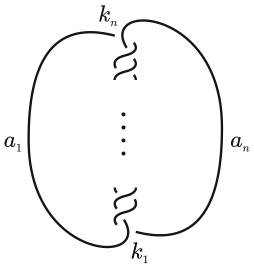
\includegraphics[scale=0.5]{3/images/5}
   \end{center}
   
   
   Zauważmy wpierw, że współczynnikiem przy wyrazie najniższego stopnia - wyrazie wolnym jest wyznacznik macierzy uzyskanej
   przez podstawienie $t =0$.
   Wtedy wynik to $1$. Współczynnik przy wyrazie najwyższego stopnia jest wyznacznikiem macierzy zawierającej
   jedynie $t$ wyrażeń w powyższej macierzy, tzn przez usunięcie wszystkich $\pm 1$. Ostatecznie wyznacznik wynosi $t^n-1$.  

   $\newline$

   Stąd wielomian Alexandera dla węzła typu $(2,n)$-torus jest stopnia dokładnie $n-1$.
   W szczególności węzły te tworzą niekończoną rodzinę rozłącznych węzłów, z czego każdy jest rozróżniany
   przez wielomian Alexandera.
\end{przyklad}

\begin{twierdzenie}
   Niech $L$ będzie zorientowany węzłem.

   \begin{enumerate}
      \item $\Delta_{mL}(t) = \Delta_{L}(t^{-1})$
      \item $\Delta_{rL}(t) = \Delta_{L}(t^{-1})$
   \end{enumerate}
\end{twierdzenie}

\begin{proof}
   Aby udowodnić $1)$ ustalmy diagram $D$ węzła $L$ i odbijmy go względem pionowej osi symetrii. Otrzymamy diagram $mD$ węzła $mL$. Weźmy
   dowolne skrzyżowanie diagramu $D$ i rozważmy odpowiadające temu skrzyżowanie w $mD$.
   
   \begin{center}
   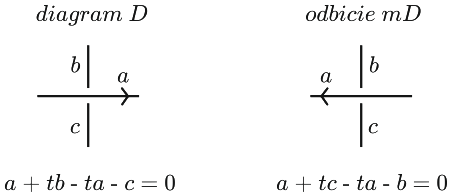
\includegraphics[scale=0.5]{3/images/6}
   \end{center}

   Współczynniki równania po lewo definiują macierz, której wyznacznik wynosi $\Delta_L(t)$ i jeżeli zastąpimy $t$ przez $t^{-1}$ dostaniemy macierz $P$, której wyznacznikiem jest $\Delta_L(t^{-1})$.
   
   Podobnie współczynniki równania po prawej stronie wyznaczają macierz $Q$, której wyznacznik to $\Delta_{mL}(t)$. Teraz zauważmy, że równanie po lewej z $t$ zastąpionym przez $t^{-1}$ jest dokładnie
   równaniem po prawej stronie pomnożonym przez $-t^{-1}$. Wtedy $P = -t^{-1} Q$ oraz
   
   $$
   \Delta_L(t^{-1}) = \det(P) = (-t)^{-m}\det(Q) = (-t^{-1})^{m}\Delta_{mL}(t) \stackrel{\bullet}{=} \Delta_{mL}(t)
   $$

   jest spełnione. 
   
   $\newline$
   
   Dowód $2)$ jest analogiczny.
\end{proof}


%--------------------------------------


\subsection{Suma spójna}

\begin{twierdzenie}
   Niech $J$ i $K$ będą zorientowanymi węzłami. Wtedy $\Delta_{J\#K}(t) \stackrel{\bullet}{=} \Delta_J(t) \Delta_K(t)$
\end{twierdzenie}

\begin{proof}
   Ustalmy diagramy dla węzłów $J$ i $K$ jak pokazano poniżej. Bez straty ogólności możemy poetykietować łuki i skrzyżowania zgodnie ze wskazanymi na Rysunku 7.

   \begin{center}
   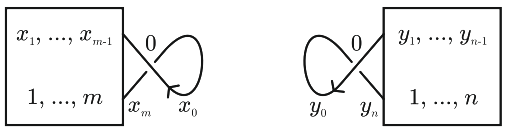
\includegraphics[scale=0.5]{3/images/7}
   \end{center}
   
   Oznaczmy przez $A$ i $B$ macierze powstałe z wielomianów rownania kolorujacego dla $J$ i $K$. Usuńmy pierwszy wiersz i pierwszą kolumnę w każdym przypadku. Wtedy
   
   $$
   \Delta_J(t) = \det(A), \qquad 
   \Delta_K(t) = \det(B)
   $$
   
   Otrzymaliśmy poniższy diagram dla $J\#K$.
     
   \begin{center}
   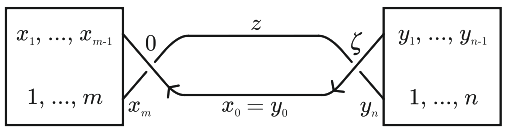
\includegraphics[scale=0.5]{3/images/8}
   \end{center}

   Mamy następujące łuki: $x_0 = y_0, x_1, \cdots, x_m, y_1, \cdots, y_m, z$, oraz skrzyżowania: $0, 1, \cdots, m$ z wezła $J$, następnie $1, \cdots, n$ z węzła $K$ oraz $\zeta$.
   Równania w węźle $J\#K$ w skrzyżowaniach $1, \cdots, m$ są dokładnie takie jak w węźle $J$, a dla skrzyżowań $1, \cdots , n$ takie jak w $K$. Dla skrzyżowania
   $\zeta$ równianie to ma postać $(1-t)y_0 + tz - y_n = 0$. 
   To pokazuje, ze jest $\Delta_{J\#K}(t)$ wyznacznikiem macierzy
   
   $$
   \begin{pmatrix}
   A & \cdots & A &  &  \\
   \vdots & \vdots & \vdots  &  \\
   A & \cdots & A &  & \\
    &  &  & B & \cdots & B  \\
    &  &  & \vdots  & \vdots & \vdots & \\
    &  &  & B & \cdots & B  \\
    &  &  &  &  & -1 & t
   \end{pmatrix}
   $$
   
   Tutaj również usuwamy pierwszy wiersz i kolumnę. Wtedy spełnione jest równanie:
   
   $$
   \Delta_{J\#K}(t) = t \Delta_{J}(t) \Delta_{K}(t) \stackrel{\bullet}{=} \Delta_{J}(t) \Delta_{K}(t)
   $$
\end{proof}


%--------------------------------------


\subsection{Równoważna defnicja}

\begin{definicja}
   Jak wspomniano wcześniej wielomiany Alexandera można wprowadzić na kilka sposobów. W tej pozycji chodziło o to, by zrobić to elementarnie. Innym sposobem 
   jest skonstruowanie funkcji $\Delta: \mathbb{L} \to \mathbb{Z}(t^{\pm 1/2})$ takiej, że dla dwóch równoważnych węzłów $L_1, L_2$ mamy równość $\Delta_{L_1} = \Delta_{L_2}$ oraz spełniającej:

   \begin{enumerate}
      \item $\Delta(   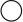
\includegraphics[scale=0.5]{3/images/l2}    ) = 1$
      \item  $\Delta(L_+) - \Delta(L_-) + (t^{1/2} - t^{-1/2})\Delta(L_0) = 0$, gdzie
         
         \begin{center}
         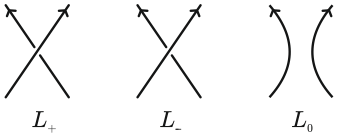
\includegraphics[scale=0.5]{3/images/9}
         \end{center}

   \end{enumerate}

   gdzie $\mathbb{L}$ oznacza zbiór wszystkich węzłów. Zobaczymy kilka przykładów:
\end{definicja}

\begin{przyklad}
   Znajdziemy wielomian Alexandera rozłącznej sumy dwóch niewęzłów, tak jak $\Delta( 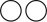
\includegraphics[scale=0.5]{3/images/l1} )$.
   Oznaczymy ten węzeł jako $L_0$ i skorzystamy z własności $2)$.

   $$
   0 = \Delta(L_+) - \Delta(L_-) + (t^{1/2} - t^{-1/2}) \Delta(L_0)
   $$ $$
   0 = \Delta (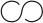
\includegraphics[scale=0.5]{3/images/l3}) - \Delta (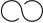
\includegraphics[scale=0.5]{3/images/l4}) + (t^{1/2} - t^{-1/2}) \Delta(L_0)
   $$ $$
   0 = \Delta (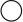
\includegraphics[scale=0.5]{3/images/l2}) - \Delta (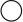
\includegraphics[scale=0.5]{3/images/l2}) + (t^{1/2} - t^{-1/2}) \Delta(L_0)
   $$ $$
   0 = (t^{1/2} - t^{-1/2}) \Delta(L_0)
   $$

   i stąd otrzymujemy, że $\Delta(L_0) = 0$.
\end{przyklad}

\begin{przyklad}
   Znajdziemy wielomian Alexandera węzła Hopfa, czyli $\Delta( 
\includegraphics[scale=0.5]{3/images/l5} )$. 
   Oznaczymy ten węzeł jako $L_+$ i
   skorzystamy z własności $2)$ na górnym skrzyżowaniu oraz z pierwszego przykładu.

   $$
   0 = \Delta(L_+) - \Delta(L_-) + (t^{1/2} - t^{-1/2}) \Delta(L_0)
   $$ $$
   0 = \Delta(L_+) - \Delta( 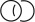
\includegraphics[scale=0.5]{3/images/l6} ) + (t^{1/2} - t^{-1/2}) \Delta( 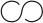
\includegraphics[scale=0.5]{3/images/l3} )
   $$ $$
   0 = \Delta(L_+) - \Delta(L_-) + (t^{1/2} - t^{-1/2}) \Delta( 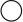
\includegraphics[scale=0.5]{3/images/l2} )
   $$ $$
   0 = (t^{1/2} - t^{-1/2}) \Delta(L_0)
   $$

   i stąd otrzymujemy, że $\Delta( 
\includegraphics[scale=0.5]{3/images/l5} ) = t^{1/2} - t^{-1/2}$.
\end{przyklad}


